\section{Синтез речи документов (вариант 8)}
\label{sec:speech}

\subsection{Постановка задачи}

В соответствии с вариантами~8 и~7 система расширена подсистемой
синтеза речи (text-to-speech, TTS) для чтения вслух документов на
\textbf{английском} и \textbf{французском} языках. Тематика корпуса "--- литературные
эссе; синтез выполняется \textbf{полностью офлайн}: без обращения к облачным
API, сетевые вызовы при генерации отсутствуют. Требования варианта:

\begin{itemize}
	\item два языка "--- \textbf{EN} и \textbf{FR};
	\item офлайн-движки, поставляемые с образом: нейросетевой \textbf{Piper}
	      (ONNX-модели, $\approx$63~МБ каждая) и формантный \textbf{eSpeak-NG}
	      (CLI, резервный);
	\item 7 голосов: 4 нейро (Siwis~F, Tom~M, Amy~F, Lessac~M)
	      и 3 формантных (fr-fr, en-us, en-gb);
	\item параметры воспроизведения: темп (rate), громкость (volume),
	      высота тона (pitch);
	\item автоматический подбор голоса по определённому языку "--- реюз
	      подсистемы распознавания языка (вариант~7, голосование большинства).
\end{itemize}

Подсистема встроена в существующую клиент-серверную архитектуру:
статическая страница \texttt{tts.html}, REST-эндпоинты, сервисный слой
и слой движков; таблицы БД не изменяются.

\subsection{Архитектура подсистемы}

Подсистема реализована шестью модулями (каталог \texttt{backend/}):

\begin{itemize}
	\item \texttt{tts/voices.py} "--- реестр голосов (id, язык, пол, движок,
	      модель), дефолтные голоса по языку, границы параметров,
	      лимит текста 4000 символов;
	\item \texttt{tts/normalize.py} "--- нормализация текста под литературный
	      домен (HTML/markdown "--- чистый текст, тире "--- пауза-запятая,
	      типографические кавычки, многоточие, схлопывание пробелов);
	\item \texttt{tts/engines.py} "--- диспетчер движков: кэш ONNX-моделей
	      Piper с блокировкой, \texttt{SynthesisConfig}, вызов
	      \texttt{espeak-ng} CLI, расчёт длительности WAV;
	\item \texttt{services/tts\_service.py} "--- валидация и клампинг
	      параметров, выбор голоса (явный / по языку / автоопределение),
	      автоматический fallback на eSpeak при отсутствии ONNX-файла,
	      сборка метрик;
	\item \texttt{controllers/tts.py} "--- четыре REST-эндпоинта
	      с Blueprint-обработчиками ошибок;
	\item \texttt{frontend/tts.html} + \texttt{frontend/js/tts.js} "--- UI:
	      ввод текста, выбор голоса (группировка по языкам), слайдеры
	      rate/volume/pitch, плеер \texttt{<audio>}, карточки статистики,
	      нормализованный текст, литературные примеры EN/FR.
\end{itemize}

Архитектура подсистемы показана на рисунке~\ref{fig:tts_arch}
(исходник "--- \texttt{plantuml/architecture\_tts.puml}).

\begin{figure}[H]
	\centering
	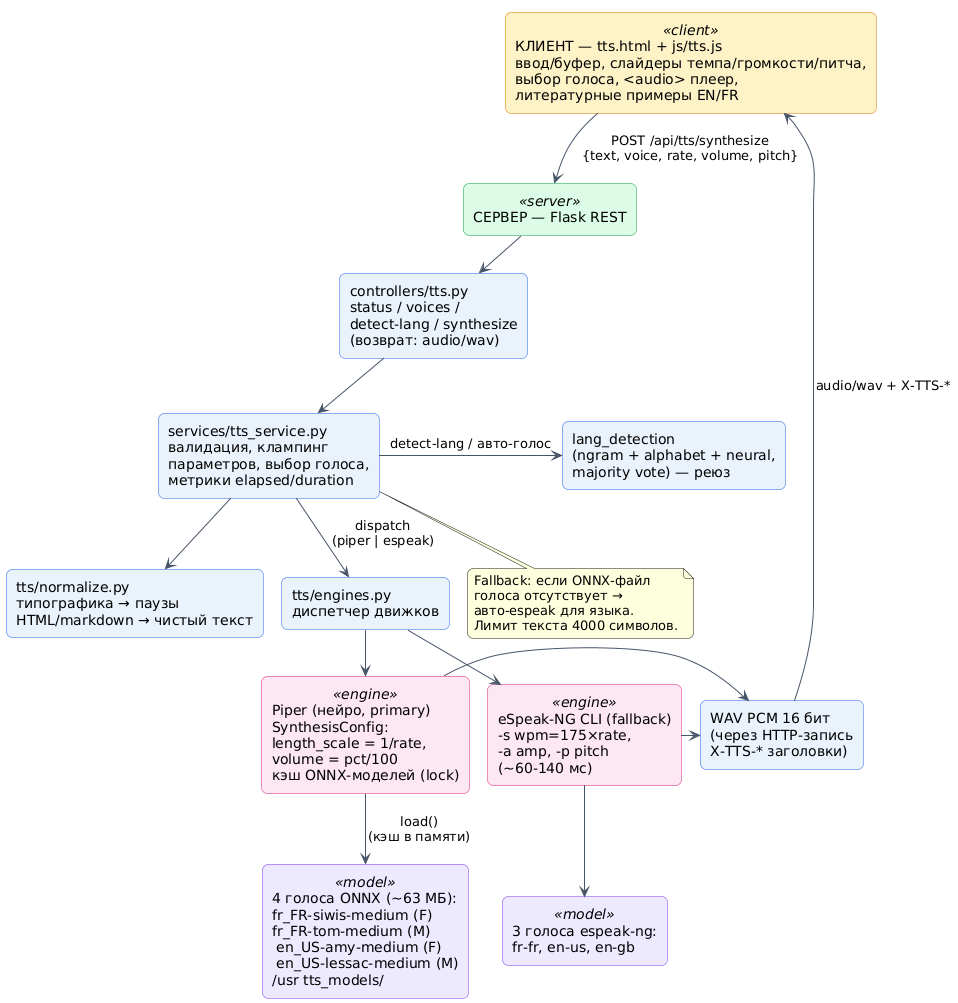
\includegraphics[width=1.0\textwidth]{png/architecture_tts.png}
	\caption{Архитектура подсистемы синтеза речи.}
	\label{fig:tts_arch}
\end{figure}

Два движка образуют единый интерфес: клиент всегда отправляет один и тот же
\texttt{POST /api/tts/synthesize}, а выбор Piper/eSpeak и параметризация
скрыты за \texttt{tts/engines.py}. Если ONNX-модель запрошенного голоса
отсутствует, сервис автоматически подменяет голос на формантный того же
языка "--- единой точкой отказа служит только отсутствие бинарника
\texttt{espeak-ng}.

\subsection{Алгоритм синтеза}

Блок-схема алгоритма приведена на рисунке~\ref{fig:tts_activity}
(исходник "--- \texttt{plantuml/activity\_tts.puml}).

\begin{figure}[H]
	\centering
	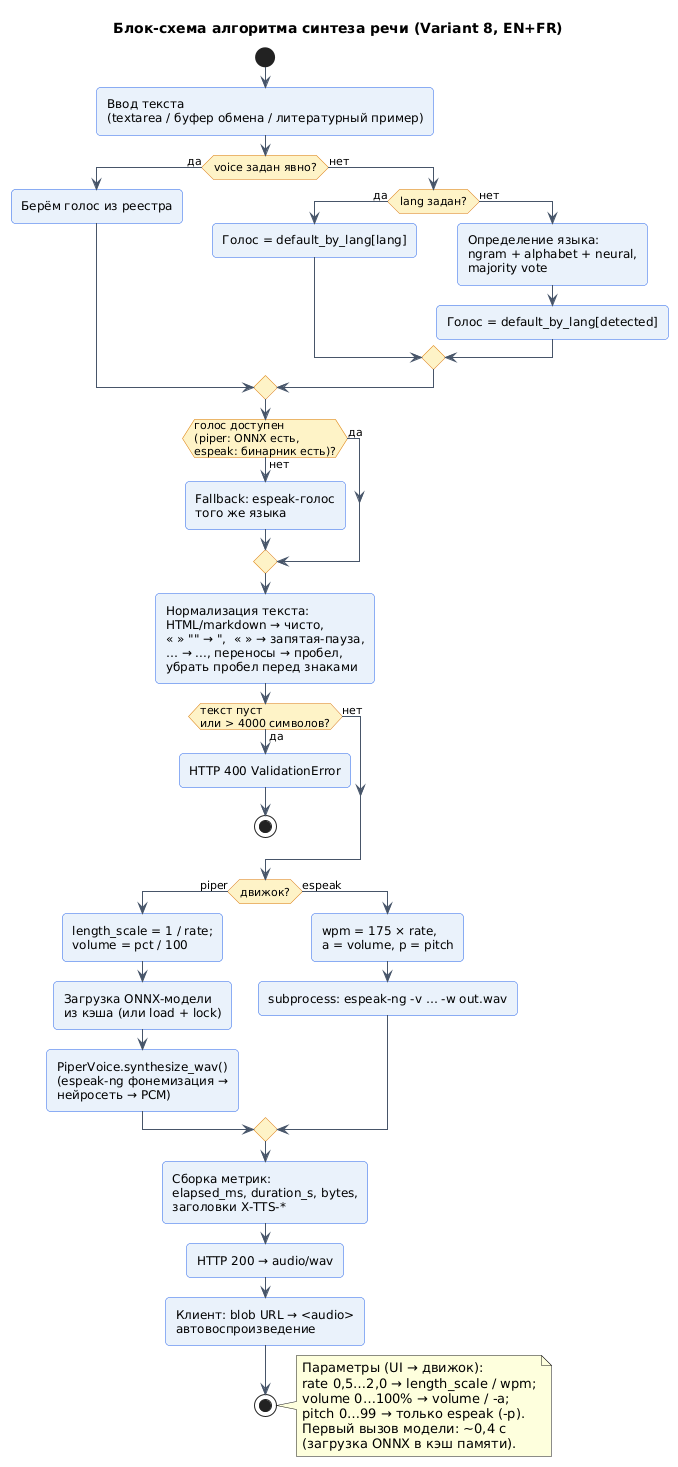
\includegraphics[width=0.85\textwidth]{png/activity_tts.png}
	\caption{Блок-схема алгоритма синтеза речи.}
	\label{fig:tts_activity}
\end{figure}

Последовательность операций:

\begin{enumerate}
	\item \textbf{Выбор голоса.} Если голос задан явно "--- берём его из
	      реестра (с валидацией id и требуемого движка). Иначе: при
	      заданном \texttt{lang} "--- дефолтный голос языка; при отсутствии
	      \texttt{lang} "--- автоопределение через
	      \texttt{classify\_text\_all} (N-граммы + алфавит + нейросеть,
	      голосование большинства, реюз варианта~7).
	\item \textbf{Проверка доступности} ONNX-файла (Piper) или бинарника
	      (eSpeak); при недоступности "--- fallback на eSpeak-голос того же
	      языка.
	\item \textbf{Нормализация} текста под литературный домен
	      (правила приведены ниже).
	\item \textbf{Валидация:} пустой текст или длиннее 4000 символов
	      "--- HTTP~400; параметры rate/volume/pitch клампятся в допустимые
	      диапазоны.
	\item \textbf{Синтез.} Piper: \texttt{length\_scale = 1/rate},
	      \texttt{volume = pct/100}, модель берётся из кэша памяти
	      (блокировка потоков); eSpeak: CLI
	      \texttt{-s wpm=175$\times$rate -a amp -p pitch -w out.wav}
	      (сериализация вызовов через lock, таймаут 60~с).
	\item \textbf{Метрики:} длительность WAV из заголовка кадров,
	      время генерации, размер; возврат \texttt{audio/wav} с
	      заголовками \texttt{X-TTS-*}.
\end{enumerate}

Сценарий вызова "--- диаграмма последовательности на
рисунке~\ref{fig:tts_seq} (исходник "---
\texttt{plantuml/sequence\_tts.puml}).

\begin{figure}[H]
	\centering
	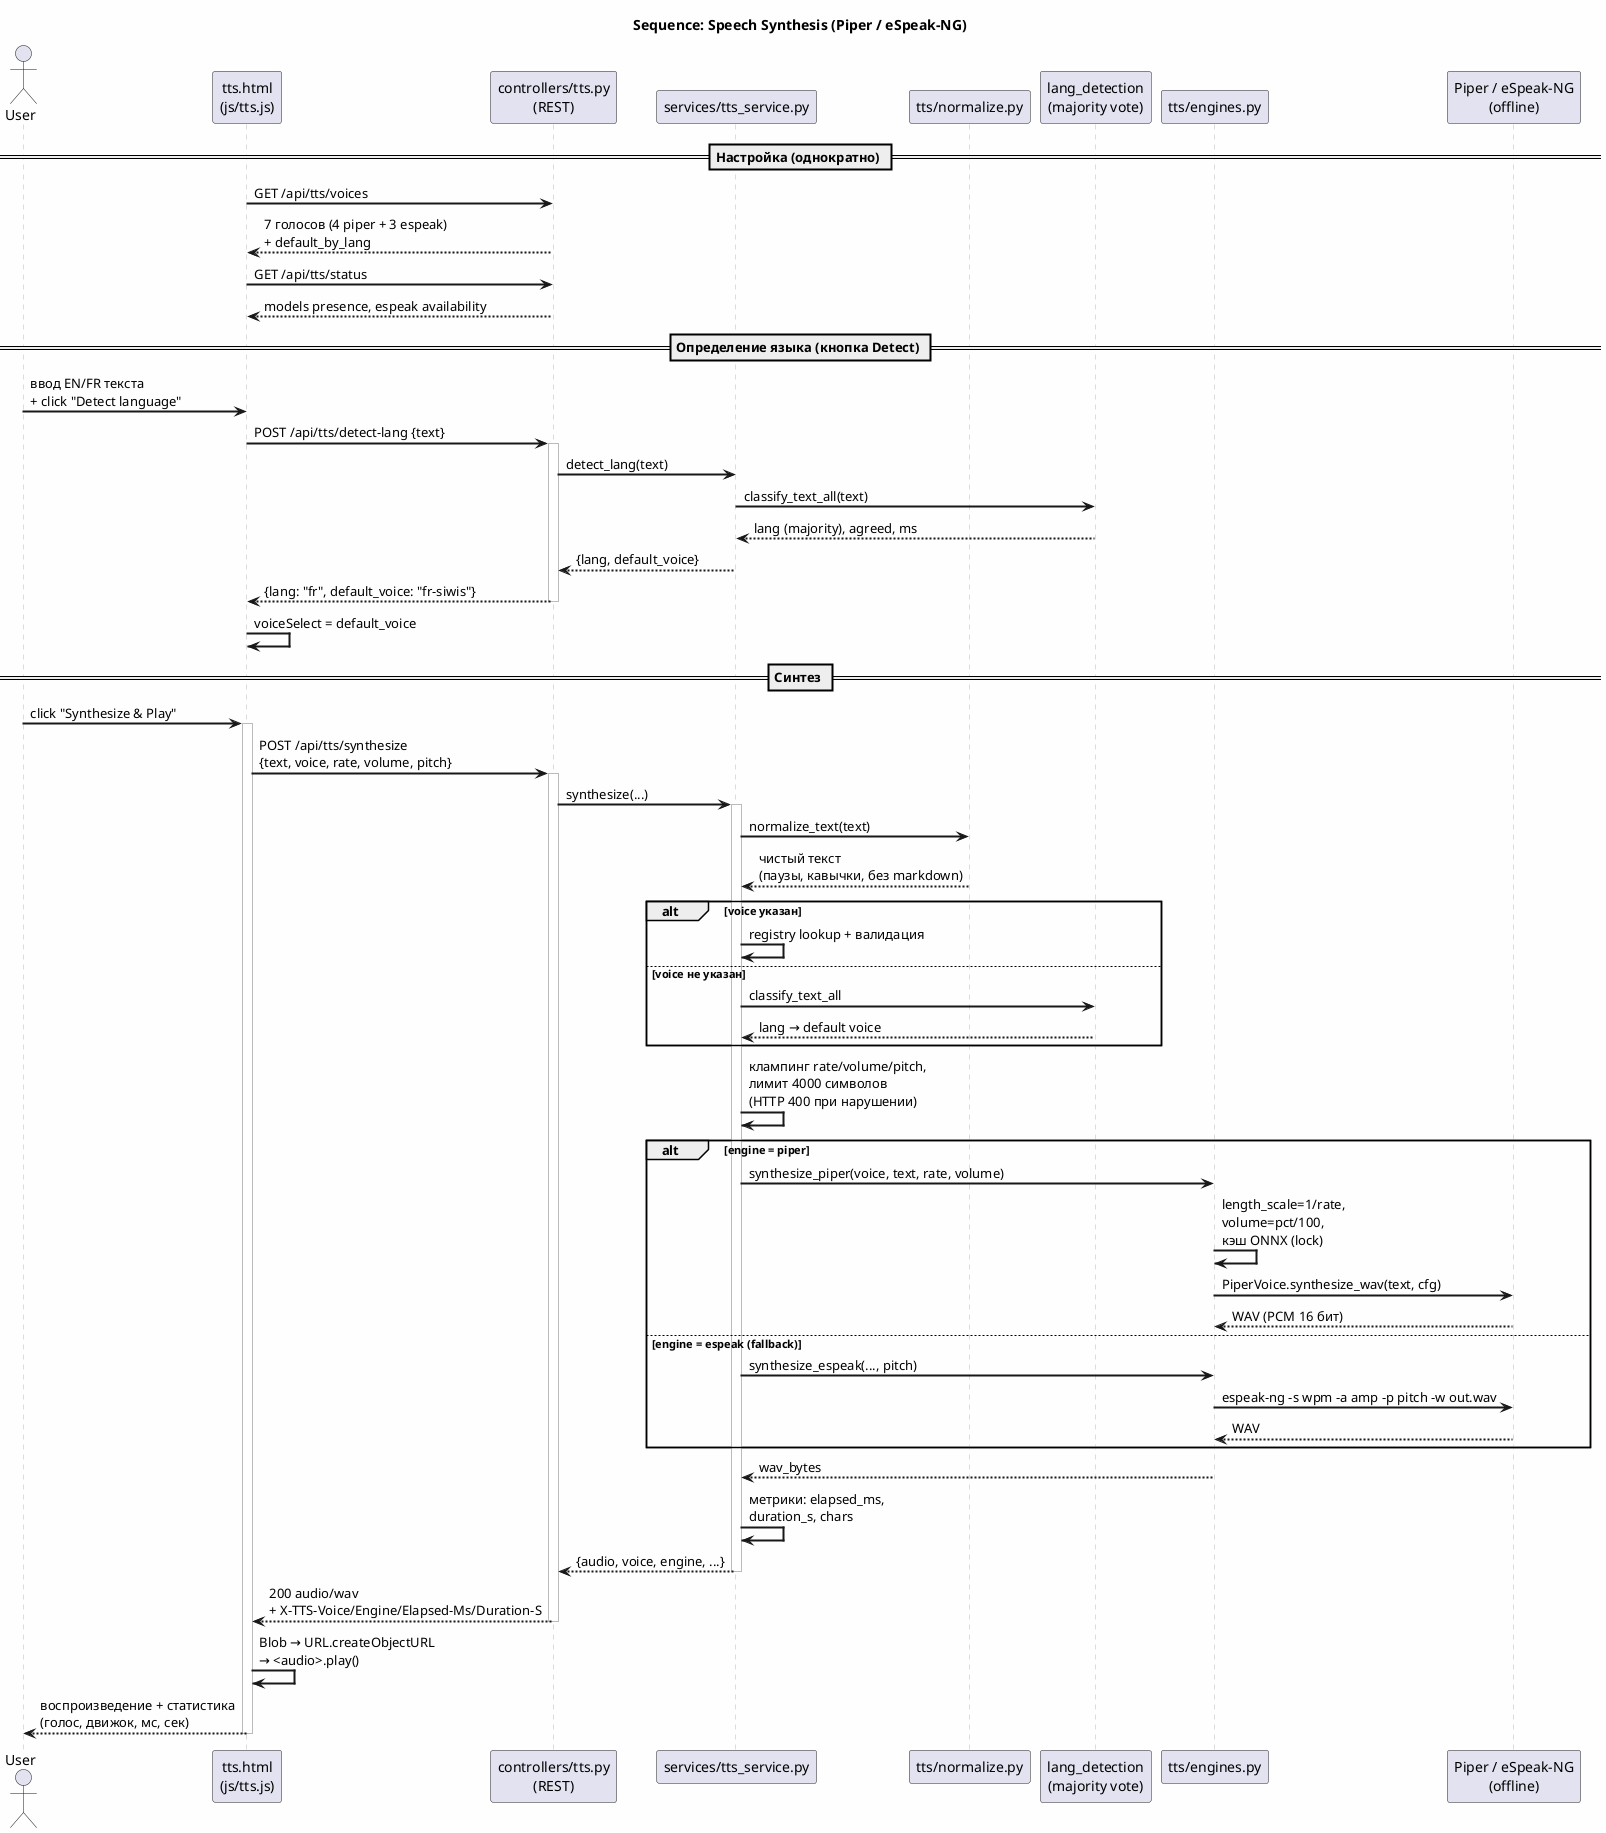
\includegraphics[width=1.0\textwidth]{png/sequence_tts.png}
	\caption{Диаграмма последовательности: синтез речи.}
	\label{fig:tts_seq}
\end{figure}

\subsection{Соответствие параметров UI и движков}

Параметры веб-интерфейса приводятся к параметрам движков
в таблице~\ref{tab:tts_params}.

\begin{table}[H]
	\caption{Маппинг параметров UI $\to$ движок.}
	\label{tab:tts_params}
	\begin{tabular}{|p{0.14\textwidth}|p{0.14\textwidth}|p{0.30\textwidth}|p{0.30\textwidth}|}
		\hline
		Параметр & Диапазон & Piper & eSpeak-NG \\ \hline
		rate (темп) & 0,5…2,0 & \texttt{length\_scale} $= 1/\mathrm{rate}$ &
			\texttt{-s wpm} $= 175 \times \mathrm{rate}$ (80…450) \\
		volume (громкость) & 0…100\,\% & \texttt{volume} $= \mathrm{pct}/100$ &
			\texttt{-a} (0…200) \\
		pitch (питч) & 0…99 & не поддерживается (возвращается \texttt{null}) &
			\texttt{-p} (0…99) \\
		текст & $\le$ 4000 символов & --- & --- \\ \hline
	\end{tabular}
\end{table}

Нормализатор \texttt{tts/normalize.py} выполняет правила,
адаптированные к литературным эссе: HTML-теги и markdown-декорации удаляются;
тире и длинное тире переводятся в запятую (короткая пауза чтения);
\texttt{…} "--- в \texttt{...}; типографические кавычки
\texttt{« » "" ''} "--- в прямые; схлопываются пробелы, переносы строк
и пробел перед знаками препинания "--- чтобы движки читали с естественными
паузами без ``залипаний'' на типографике.

\subsection{API методы}

\begin{lstlisting}[caption={HTTP эндпоинты подсистемы синтеза речи.},label={lst:tts_api}]
GET  /api/tts/status       --- доступность Piper/eSpeak, наличие моделей
GET  /api/tts/voices       --- 7 голосов + default_by_lang
POST /api/tts/detect-lang  --- автоопределение языка текста (EN/FR)
POST /api/tts/synthesize   --- синтез: text, voice, lang, rate, volume, pitch
                               => 200 audio/wav + X-TTS-* заголовки
\end{lstlisting}

Заголовки ответа \texttt{X-TTS-Voice}, \texttt{X-TTS-Engine},
\texttt{X-TTS-Lang}, \texttt{X-TTS-Elapsed-Ms}, \texttt{X-TTS-Duration-S},
\texttt{X-TTS-Chars}, \texttt{X-TTS-Normalized} позволяют клиенту
показать статистику без дополнительного запроса.

\subsection{Интерфейс пользователя}

Страница \texttt{tts.html} (пункт меню ``Speech'') содержит: поле ввода
текста (с вставкой из буфера), выпадающий список голосов с группировкой
по языкам и пометкой движка, кнопки ``Detect language'' и
``Synthesize \& Play'', слайдеры темпа/громкости/питча, HTML5-плеер,
карточки статистики (голос, движок, задержка, длительность, символы),
блок нормализованного текста и четыре литературных примера
(Бодлер, Ламартин, Уайльд, Шекспир). Страница ``Help'' дополнена
разделом ``Speech Synthesis Theory'' с описанием методов TTS.

\subsection{Тестовые результаты}

Все замеры выполнены в контейнере \texttt{app} (CPU-only, Docker)
на абзаце французского текста (555 символов), если не указано иное;
полный результат сохранён в \texttt{/tmp/tts\_bench.json}.

Задержка генерации и размер WAV в зависимости от длины текста
(Piper \texttt{fr-siwis}, тёплый кэш модели) "--- таблица~\ref{tab:tts_len}.

\begin{table}[H]
	\caption{Задержка и объём WAV по длине текста (Piper, fr-siwis).}
	\label{tab:tts_len}
	\begin{tabular}{|l|l|l|l|l|}
		\hline
		Текст & Символов & Задержка & Длительность WAV & Размер \\ \hline
		короткое предложение & 22 & 0,26~с & 1,59~с & 68~КБ \\
		абзац & 555 & 4,0~с & 30,8~с & 1,3~МБ \\
		длинный фрагмент & 2220 & 16,7~с & 121,7~с & 5,2~МБ \\ \hline
	\end{tabular}
\end{table}

Задержка растёт практически линейно с длиной текста
($\approx$7,5~мс на символ); отношение длительности WAV к задержке
$\approx$7--8 остаётся стабильным, что позволяет планировать
стриминговую выдачу для длинных документов.
Первый (``холодный'') вызов после перезапуска занимает 0,38~с "--- загрузка
ONNX-модели в кэш памяти; далее вызовы идут по тёплому кэшу.

Влияние темпа на длительность речи "--- таблица~\ref{tab:tts_rate}.

\begin{table}[H]
	\caption{Влияние параметра rate на длительность (555 символов, Piper).}
	\label{tab:tts_rate}
	\begin{tabular}{|l|l|l|l|}
		\hline
		rate & Длительность & Отношение к 1,0 & Задержка \\ \hline
		0,5 & 54,6~с & 1,57 & 6,7~с \\
		1,0 & 30,8~с & 1,00 & 4,1~с \\
		1,5 & 22,3~с & 0,72 & 3,1~с \\
		2,0 & 18,6~с & 0,60 & 2,7~с \\ \hline
	\end{tabular}
\end{table}

Полуторное снижение длительности при rate~=~0,5 и двукратное ускорение
при rate~=~2,0 подтверждают корректность преобразования
\texttt{length\_scale} $= 1/\text{rate}$ (нелинейность вблизи пределов
объясняется фиксированными паузами между предложениями).
Громкость проверена по RMS-амплитуде WAV: 5155 при 100\,\%
против 1498 при 30\,\% "--- монотонное уменьшение подтверждено.

Сравнение голосов (тот же абзац, тёплый кэш) "--- таблица~\ref{tab:tts_voices}.

\begin{table}[H]
	\caption{Сравнение голосов: задержка / длительность / размер.}
	\label{tab:tts_voices}
	\begin{tabular}{|l|l|l|l|}
		\hline
		Голос & Движок & Задержка & Длительность / размер \\ \hline
		fr-siwis (F) & Piper & 4,07~с & 30,6~с / 1,3~МБ \\
		fr-tom (M) & Piper & 6,87~с & 33,3~с / 2,9~МБ \\
		espeak-fr & eSpeak & \textbf{0,07~с} & 25,5~с / 1,1~МБ \\ \hline
		en-amy (F) & Piper & 2,97~с & 22,0~с / 948~КБ \\
		en-lessac (M) & Piper & 2,79~с & 18,1~с / 779~КБ \\
		espeak-en-us & eSpeak & \textbf{0,06~с} & 19,0~с / 819~КБ \\
		espeak-en-gb & eSpeak & \textbf{0,06~с} & 18,5~с / 796~КБ \\ \hline
	\end{tabular}
\end{table}

Нейро-голоса Piper генерируют естественную речь с задержкой
2,8--6,9~с на абзац; формантные голоса eSpeak "--- за 60--70~мс
(в $\approx$50 раз быстрее) при синтетическом тембре, что делает их
пригодными как fallback и для быстрого прослушивания.
Два французских нейро-голоса различаются и по длительности
(30,6 против 33,3~с), и по ритму чтения "--- выбор голоса влияет
на подачу текста.

Определение языка (реюз варианта~7) на контрольных примерах:
EN "--- 29,6~мс, FR "--- 4,7~мс, в обоих случаях все три метода
сошлись (\texttt{agreed=true}), дефолтные голоса
\texttt{en-amy}/\texttt{fr-siwis} выбраны корректно.
Контроль ошибок: пустой текст, неизвестный id голоса и текст длиннее
4000 символов корректно возвращают HTTP~400 с сообщением
\texttt{ValidationError} через Blueprint-обработчик.

\subsection{Выводы}

Реализована подсистема офлайн-синтеза речи для EN и FR
(вариант~8): единый REST-интерфейс поверх двух движков "---
нейросетевого Piper и формантного eSpeak-NG, 7 голосов,
параметры темп/громкость/питч с корректным маппингом на
\texttt{length\_scale}/CLI-флаги, нормализация литературного текста,
автоопределение языка и подбор голоса реюзом подсистемы
распознавания языка, fallback при отсутствии моделей.
Тесты подтвердили линейный рост задержки по длине текста,
корректное влияние темпа на длительность, монотонность громкости
и работоспособности всех семи голосов. Направления улучшения:
поблочный (стриминговый) синтез длинных документов, кэш WAV
в MinIO, SSML-паузы для абзацев, оценка естественности (MOS),
поддержка pitch в Piper и чтение документов по найденным фрагментам.
